\documentclass{article}
\usepackage[margin=1in, top = .8in, left=.8in]{geometry}
\usepackage{comment}
\usepackage{amsmath, amssymb}
\usepackage{framed}
\usepackage{enumerate}
\usepackage{comment}
\usepackage{tikz,pgfplots}
\usepgfplotslibrary{fillbetween}
\pgfplotsset{compat=1.15}
\usepackage[hyphens]{url}

\begin{document}

\begin{center}
    \large \textbf{Homework 5}
\end{center}
    %\item[\textbf{Week 5}]
        \begin{itemize}
            %\item Sync (Week 4):
            \item Part 1
                \begin{enumerate}

    \item Review question: in class you found the area of the shaded region in the graph below. The function shown is $f(x) = 4x-x^3$. Use the techniques of calculus to find the height of the high point of the region. Then use this value to do a ``sanity check'' of the value for the area that you found in class, by noting that the exact area should be slightly higher than the area of the triangle inscribed within the region.
\begin{center}
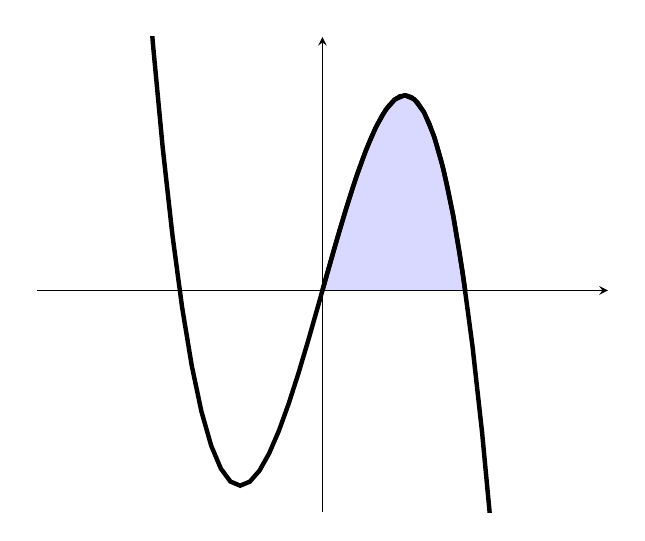
\begin{tikzpicture}
\begin{axis}[
   	xmin=-4, xmax=4,
	ymin=-3.5, ymax=4,
%	xtick={2,4,6,8,10},  
%	ytick={2,4,6,8,10,12},
    yticklabels={,,},
    xticklabels={,,},
	major tick length={0},
	line width=1pt,
 	axis lines=center, height=3 in,
	]
    \addplot [ultra thick, samples=60,domain=-4:4] {4*x-x^3};
    \addplot [name path = f,ultra thick, domain=0:2] {4*x-x^3};
       \path[name path=axis] (axis cs:0,0) -- (axis cs:4,0);
    \addplot [
        thick,
        color=blue,
        fill=blue, 
        fill opacity=0.15
    ]
    fill between[
        of=f and axis
    ];
\end{axis}
\end{tikzpicture}
\end{center}

    \item Evaluate the following definite integrals. The answer should be a number. If you cannot give an exact value, then give its value to within exactly four decimal points. 
    \begin{enumerate}
        \item $\displaystyle \int_{-1}^{2} \frac{2}{5}z^9-{1}{4}z^3 + 3z + 1 \, dz$
        \item $\displaystyle \int_1^9 \frac{\sqrt{t}-1}{t^{\frac{3}{2}}}\,dt$
        \item $\displaystyle \int_0^1 p(\sqrt[3]{p}+\sqrt[4]{p})\,dp$
        \item $\displaystyle \int_{0}^{2} \left| 2x-1
        \right|\,dx$
        \item $\displaystyle \int_0^1 (b^2+2)^4\,db$
    \end{enumerate}

    \item The graph below shows a function $f(x) = cx(x-b)^2$. Find the value of $c$ so that the shaded blue area is equal to 1. Note that choosing the values of the parameters so that the area under the curve is 1 means that we can use this function, restricted to the appropriate domain, as a probability density function. After finding the value of $c$, use it to find the probability that a random variable with this density function lies between 0 and $\displaystyle \frac{b}{2}$.
    \begin{center}
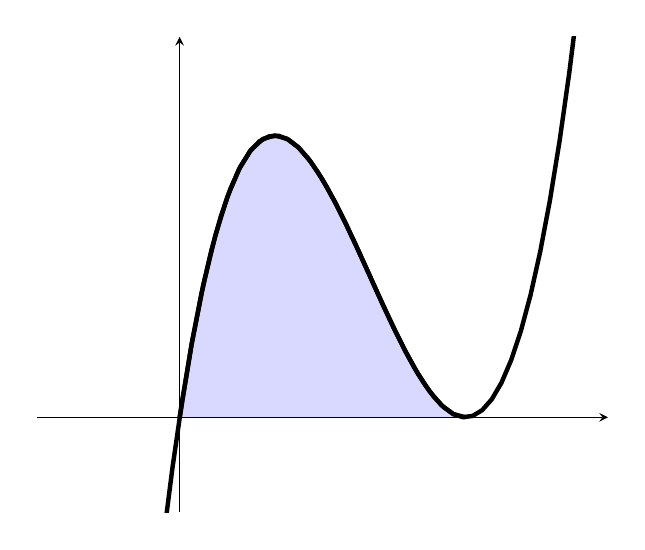
\begin{tikzpicture}
\begin{axis}[
   	xmin=-.5, xmax=1.5,
	ymin=-0.5, ymax=2,
%	xtick={2,4,6,8,10},  
%	ytick={2,4,6,8,10,12},
    yticklabels={,,},
    xticklabels={,,},
	major tick length={0},
	line width=1pt,
 	axis lines=center, height=3 in,
	]
    \addplot [ultra thick, samples=60,domain=-.5:1.5] {10*x*(x-1)^2};
    \addplot [name path = f,ultra thick, domain=0:1] {10*x*(x-1)^2};
       \path[name path=axis] (axis cs:0,0) -- (axis cs:1,0);
    \addplot [
        thick,
        color=blue,
        fill=blue, 
        fill opacity=0.15
    ]
    fill between[
        of=f and axis
    ];
\end{axis}
\end{tikzpicture}
\end{center}


\item  The function $\displaystyle f(x) = \frac{1}{\sqrt{2\pi}}e^{-\frac{x^2}{2}}$ is the probability density function for the standard normal distribution (also known as the ``bell curve.'') Use WolframAlpha (or any other
graphing technology) to graph this curve. Then use technology to find the area under the curve and above the $x$-axis on the interval $[-\infty,1]$. Repeat on the interval $[-\infty,2]$. Then use those two numbers to find the area under the curve on the intervals $[-1,1]$, $[-1, 2]$, and $[2,2]$. Shade the regions on the graph to show what you are finding the area of. These numerical answers are very important in statistics and might be familiar if you have taken a statistics class before. Note that we are not able to find a closed-form solution to the anti-derivative, so currently the best we can do is a numerical estimate of this definite integral, as we've done in this problem. Later in the course we'll see other ways to approximate these areas.
\item Say that $F(x)= \ln{x}$, and $F'(x)=f(x)$. Find $\displaystyle \int_3^2 5f(x) \,dx$.


\end{enumerate}
            %\item Async (Week 5):
            \item Part 2
                \begin{enumerate}
                    \item Given $F'(x)=f(x)$, evaluate $\displaystyle \int x^3f(2x^4)\ dx$. You may need to use $F(x)$ and/or $f(x)$ in your answer.
                    \item If $\displaystyle \int_a^b f(x)\,dx = c$, what does 
                    $\displaystyle \int_{a+6}^{b+6} f(x-6)\,dx$ equal?
                    \item If $\displaystyle \int_a^b f(x)\,dx = c$, what does 
                    $\displaystyle \int_{a/6}^{b/6} f(6x)\,dx$ equal?
                    \item Evaluate the indefinite integral 
                    $\displaystyle \int \frac{e^{\sqrt{x}}}{\sqrt{x}}\,dx$.
                    
                    \item Evaluate the definite integral 
                    $\displaystyle \int_{1}^{e} \frac{(\ln{x})^2}{x}\,dx$.
                    \item Evaluate $\displaystyle \int x\ln(x)\ dx$.  Because $\int \ln(x)\ dx$ is not obvious, the best choice to apply integration by parts is with $f(x)=\ln(x)$ and $g'(x)=x$.
                    \item Evaluate $\displaystyle \int x^4e^x\ dx$.  This will require multiple iterations of integration by parts.
                    \item Given $F'(x)=f(x)$ and $G'(x)=F(x)$, evaluate $\displaystyle \int_a^b xf(x)\ dx$, using the information on the following table. \\
                        \begin{center}
                        \begin{tabular}{|c|c|c|c|}
                        \hline
                        $x$ & $f(x)$ & $F(x)$ & $G(x)$ \\
                        \hline
                        $a$ & $2$ & $4$ & $10$ \\
                        \hline
                        $b$ & $-1$ & $5$ & $-11$ \\
                        \hline 
                        \end{tabular}
                        \end{center}
                        \medskip
                        
                    \item Find the value of $c$ so that the function 
                    $\displaystyle \frac{c\ln{x}}{x^2}$ defines a probability density function on the interval $[1,2]$. (Hint: What must the area under the curve be?)
                    
                    \item On a previous homework, you used technology to find that $\displaystyle \int_{-1}^{1} \frac{1}{\sqrt{2\pi}} \exp\left(-\frac{x^2}{2}\right)\,dx \approx 0.6827$. This shows that the probability that a standard normal random variable lies between $-1$ and $1$ is $68.27\%$. Now, without using technology, find the following integrals. Show your work.
                    $$\displaystyle \int_{-1}^{1} \frac{1}{\sqrt{2\pi}}x \exp\left(-\frac{x^2}{2}\right)\,dx$$.
                    $$\displaystyle \int_{-1}^{1} \frac{1}{\sqrt{2\pi}}x^2 \exp\left(-\frac{x^2}{2}\right)\,dx$$.
                    \item Evaluate $\displaystyle \int_{\mu-\sigma}^{\mu+\sigma} \frac{1}{\sqrt{2\pi \sigma^2}}x \exp\left(-\frac{(x-\mu)^2}{2\sigma^2}\right)\,dx$.
                    \item The function $f(x) = c\sin{x^2}$ defines a probability density function on the interval $[0, \sqrt{\pi}]$.
                    \begin{enumerate}
                        \item Use technology to estimate the value of $c$.
                        \item Using this value for $c$, find the expected value of this distribution. Evaluate the integral without using technology.
                    \end{enumerate}
                    \item Complete the Area Accumulation Function Introduction project.

                \end{enumerate}
        \end{itemize}


\end{document}